\section{Introduction}
There are myriads of ways to deform a planar sheet without stretching or tearing it. One can bend it, fold it, or combine the two. Folding and bending isometries are different by nature, and historically speaking there is some dichotomy in the study of the two; Smooth isometries are typically studied in differential geometry \cite{do_carmo}, whereas straight folds are often explored in the field of computational origami \cite{origami_book}. Curved folded surfaces \cite{huffman} result as a combination of the two, as folding an inextensible sheet along a curve necessitates global bending around the crease.

Building curved folded sculptures is a manual and time consuming process, often done using an empirical trial and error approach  as little theory is known \cite{curved_review,huffmann_reconstructing}. Contrary to classical origami, bending and folding instructions are hard to write down and the fact that multiple creases need to fold simultaneously further complicates the process \cite{StringActuated:2017}. Artists often pre-crease the paper using a ball burnisher or a CNC plotter before carefully folding and bending it, making the process of exploration even slower. 

Albeit manual, slow, and exhaustive, playing with paper is currently the only option available for an explorer of curved folds. Existing works on modeling these surfaces are either limited to previously discovered sculptures \cite{curved_folding_kilian,StringActuated:2017} or model a small partial set of folded surfaces generated by reflections or rotational sweeps \cite{Mitani_ref,mitani2009design}. Modeling the folding process of novel forms remains a challenge \cite{curved_review}. 

In this paper we set to develop the basic tools for unconstrained modeling of curved folds, set with the objective of aiding the exploration, analysis and study of new curved folded structures. Our work builds upon Discrete Orthogonal Geodesic Nets (DOGs) \cite{rabi18,rabi2018shape} as a discrete model for smooth developable surfaces. These are regular quadrilateral meshes with equal angles around each vertex, and unlike other computational models for developables do not suffer from locking of various deformation modes \cite{locking1,locking2,grin_shells}, are not fixed to predetermined rulings directions \cite{pottmann_new,curved_folding_kilian} or require remeshing while deforming the surface \cite{StringActuated:2017,SchreckEG2017,Narain}. The regularity of the DOG meshing also simplifies various curved folding objectives. We represent curved folded models as piecewise smooth developable surfaces with boundary constraints pushing for equal discrete geodesic curvature along their intersections, as done in \cite{rabi2018shape}.

In practice, deforming a piecewise DOG while keeping the geodesic boundary constraints does not usually results in a model that is folded along all creases (see \figref{fig:folded_and_not_folded}). In our "Preliminary" section we look at the smooth and combinatorial degrees of freedom of curved foldings, detailing how a flat piecewise smooth developable surface is locally a bifurcation point between folded and unfolded configurations. Folding along a crease given one side of the surface is in fact a binary choice (Add a figure). At \secref{sec:folding} we give a simple discrete charecterization for this binary choice by looking at supporting planes along the creases. This observation translates to an effective algorithm to enforce folds while deforming a piecewise DOG. We supplement that algorithm with objectives to control mountain/valley assignments and dihedral angles along folds. At \secref{sec:rulings}, we study objectives to control the rulings on curved folds, whose angles dictates singularities on developable surfaces. This exploration begins by discretizing a local notion of a second fundamental form on DOGs up to symmetry, torsions along the parameter lines, and objectives for cylindrical flow, fixing rulings direction and rotating them. We also prove a basic theorem on the local existence of rigid folding. At \secref{sec:app}, we explore a variety of applications for our tools such as wallpaper curved foldings, rigid folding, and modeling while dynamically changing the creased pattern.

\begin{figure} [h]
	\centering
	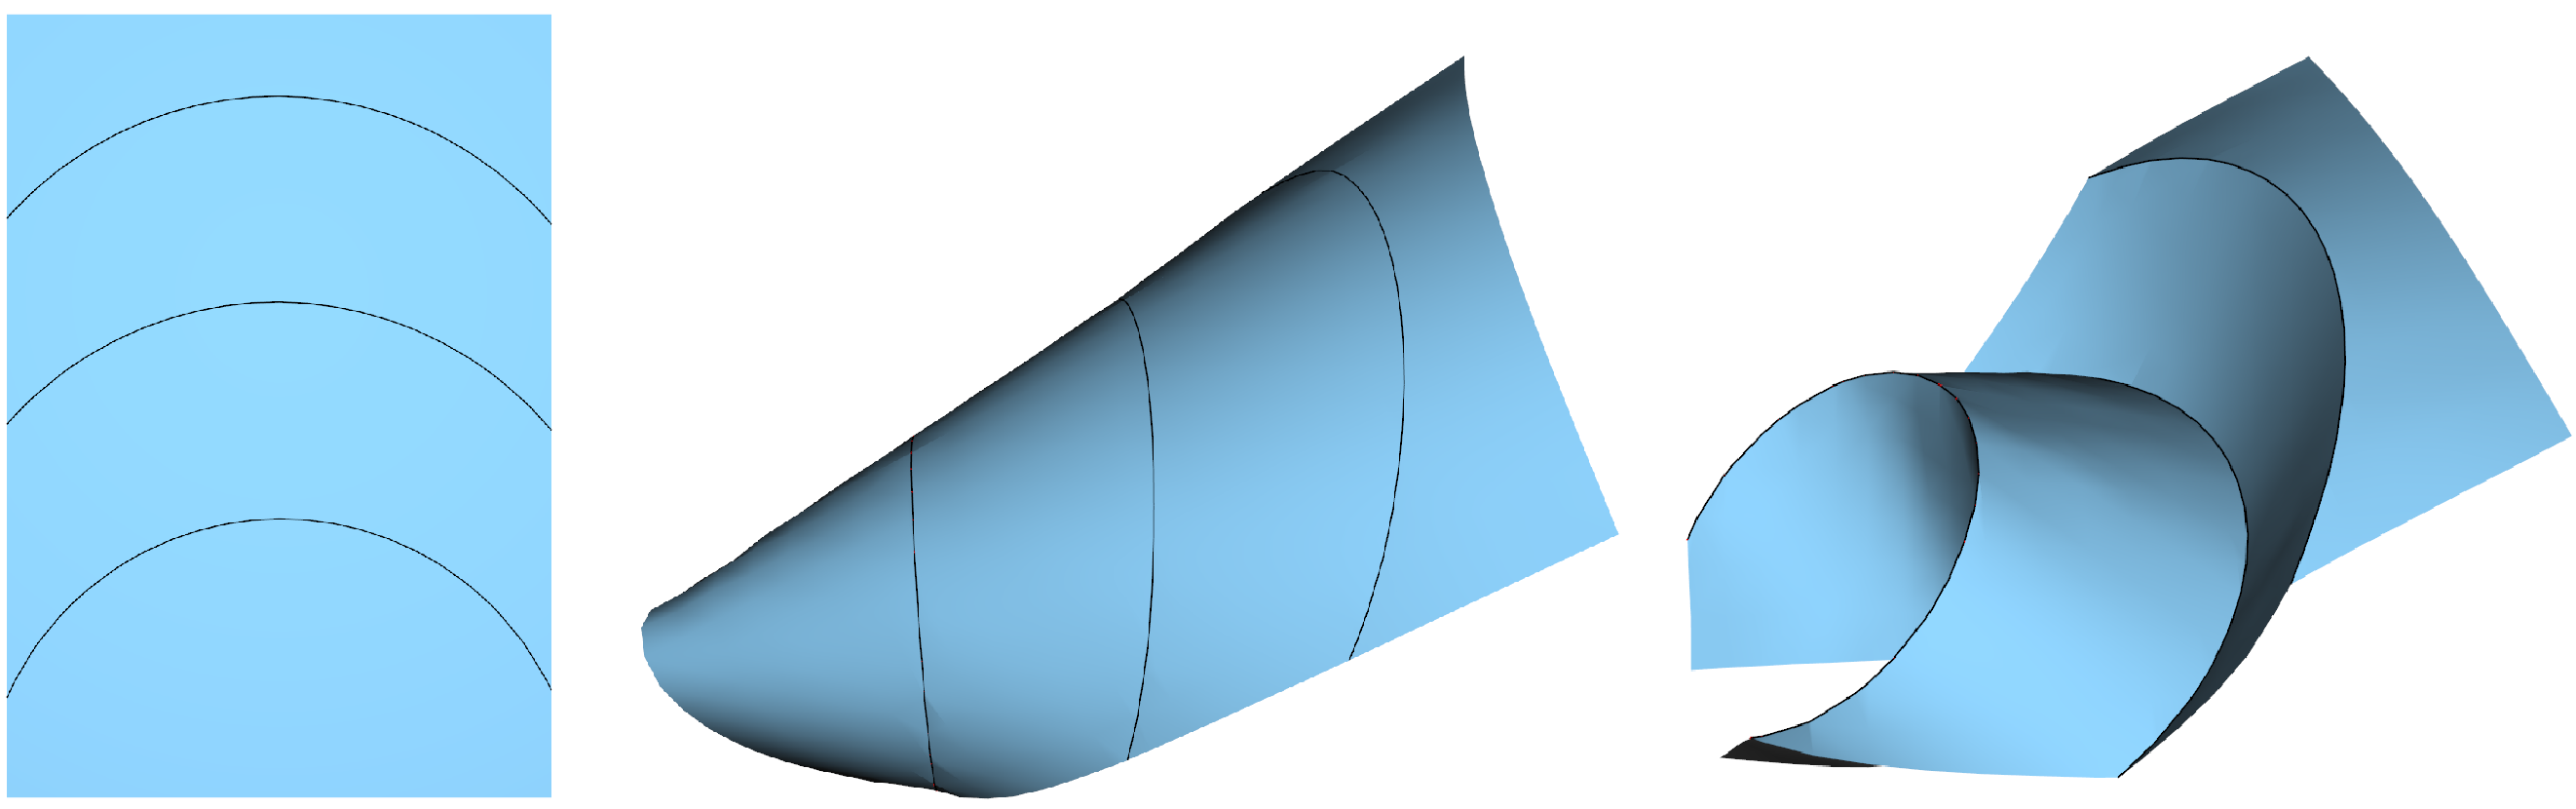
\includegraphics[width=\linewidth]{figures/folded_and_not_folded}
	\caption{TODO: caption and better normals rendering. (Same deformation, besides the bias).}
	\label{fig:folded_and_not_folded}
\end{figure}